\section{Dynamiczny przydział priorytetów}
\label{ch:alg-priorities-allocation}
Obok samego algorytmu WHCA* zrealizowano własną metodę dynamicznego przydziału priorytetów oraz skalowania okna czasowego, która to przyczynia się do zwiększenia skuteczności planowania ruchu robotów. Stanowi ona niejako rozwinięcie metody WHCA* o dodatkowe procedury.
Dla rozróżnienia poszczególnych wariantów metody WHCA* w dalszej części pracy będziemy posługiwać się skrótowymi nazwami:
\begin{itemize}
	\item {\bf WHCA*1} - {\it Windowed Hierarchical Cooperative A*} bez dynamicznego przydzielania priotytetów, ze stałym oknem czasowym,
	\item {\bf WHCA*2} - {\it Windowed Hierarchical Cooperative A*} z dynamicznym przydziałem priorytetów, ze stałym oknem czasowym,
	\item {\bf WHCA*3} - {\it Windowed Hierarchical Cooperative A*} z dynamicznym przydziałem priorytetów oraz skalowaniem okna czasowego.
\end{itemize}

Układ priorytetów w metodzie WHCA* ma znaczący wpływ na wynik planowania tras. Od priorytetów robotów zależy kolejność wyznaczania tras.
Jest to na tyle istotne, gdyż podczas wyznaczania tras uwzględniane są tylko roboty o priorytetach wyższych (których planowanie odbyło się wcześniej).

\subsection{Detekcja kolizji}
Podobnie jak w algorytmie LRA*, również w metodzie WHCA* należy wykrywać kolizje (odpowiednio wcześniej).
Nawet w przypadku, gdy roboty podążają wzdłuż zaplanowanych ścieżek, wciąż istnieje możliwość wystąpienia kolizji.
Taka sytuacja może wystąpić, gdy robot, który planuje drogę wcześniej (ma wyższy priorytet), nie uwzględnia, że następnemu robotowi może nie udać się wyznaczenie trajektorii (z powodu właśnie zaplanowanej trasy).
Wykrywanie kolizji odbywa się tak samo, jak w przypadku metody LRA* (por. \ref{ch:alg-collision-avoid}).
Należy zaznaczyć, że pod pojęciem wykrywania kolizji rozumiemy wczesne zauważenie kolizji, która wystąpiłaby w następnym kroku. Niepożądane jest doprowadzanie do faktycznych kolizji, dlatego interwencja zachodzi odpowiednio wcześniej.

% TODO screen z przypadku kolizjii

\subsection{Wariant WHCA*2}
%TODO stała wartość okna
Wariant WHCA*2 został wzbogacony o dynamiczny przydział priorytetów agentów.
Zaproponowane podejście polega na zwiększaniu priorytetów robotów w przypadku niepowodzenia w znalezieniu trasy.
Opiera się to na następujących krokach:
\begin{enumerate}
	\item Początkowo roboty mają nadane priorytety losowo. Otrzymują kolejne wartości od 1 do liczby wszystkich robotów.
	\item Rozmiar okna czasowego jest zawsze równy całkowitej liczbie agentów zwiększonej o 1.
	\item Planowanie tras dla robotów wykonywane jest w przypadku detekcji kolizji w poprzednim kroku symulacji, lub gdy robot wykonał już wszystkie akcje z jego indywidualnej kolejki akcji.
	Lista robotów zostaje posortowana malejąco według priorytetów przed wykonaniem planowania tras. Wyższa wartość priorytetu oznacza pierwszeństwo podczas planowania.
	\item Następnie wykonywane jest planowanie tras zgodnie z aktualnym układem kolejnosci robotów (jak w wariancie WHCA*1). Wyznaczone ścieżki zaznaczane są kolejno w tablicy rezerwacji.
	\item Jeśli dla któregoś robota nie została znaleziona bezkolizyjna ścieżka, to następuje zwiększenie jego priorytetu o wartość 1. Taki awans priorytetów może nastąpić dla wielu robotów w jednym kroku symulacji.
	\item Dla wszystkich robotów dokonywana jest weryfikacja wystąpienia kolizji. W przypadku jej wykrycia, kolejka ruchów obydwu (lub więcej) robotów zostaje opróżniona.
	\item W następnych krokach symulacji zostanie podjęta próba ponownego poszukiwania tras dla robotów, u których wystąpiło niepowodzenie planowania lub została wykryta kolizja. Tym razem nastąpi to z nowym układem priorytetów.
\end{enumerate}

Rozmiar okna czasowego jest stały i jest równy całkowitej liczbie agentów na mapie zwiększonej o 1.

\subsection{Wariant WHCA*3}
Wariant WHCA*3 stanowi rozszerzenie WHCA*2 o procedurę skalowania okna czasowego.
Rozmiar okna czasowego może zmieniać się w trakcie trwania symulacji.

Poniżej przedstawiono kroki wariantu WHCA*3. Modyfikacje w stosunku do wariantu WHCA*2 zostały oznaczone jako pogrubione. Wprowadzają one dodatkowe powiększanie okna czasowego do procedury dynamicznego przydziału priorytetów:
\begin{enumerate}
	\item Początkowo roboty mają nadane priorytety losowo. Otrzymują kolejne wartości od 1 do liczby wszystkich robotów.
	\item {\bf Rozmiar okna czasowego jest początkowo równy całkowitej liczbie agentów zwiększonej o 1.}
	\item Planowanie tras dla robotów wykonywane jest w przypadku detekcji kolizji w poprzednim kroku symulacji, lub gdy robot wykonał już wszystkie akcje z jego indywidualnej kolejki akcji.
	Lista robotów zostaje posortowana malejąco według priorytetów przed wykonaniem planowania tras. Wyższa wartość priorytetu oznacza pierwszeństwo podczas planowania.
	\item Następnie wykonywane jest planowanie tras zgodnie z aktualnym układem kolejnosci robotów (jak w wariancie WHCA*1). Wyznaczone ścieżki zaznaczane są kolejno w tablicy rezerwacji.
	\item Jeśli dla któregoś robota nie została znaleziona bezkolizyjna ścieżka, to następuje zwiększenie jego priorytetu o wartość 1. Taki awans priorytetów może nastąpić dla wielu robotów w jednym kroku symulacji.
	\begin{enumerate}
		\item {\bf Jeśli nowa wartość priorytetu robota przekracza aktualną wartość rozmiaru okna czasowego, to okno czasowe zostaje zwiększone do wartości równej maksymalnemu priorytetowi robota.}
	\end{enumerate}
	\item Dla wszystkich robotów dokonywana jest weryfikacja wystąpienia kolizji. W przypadku jej wykrycia, kolejka ruchów obydwu (lub więcej) robotów zostaje opróżniona.
	\item W następnych krokach symulacji zostanie podjęta próba ponownego poszukiwania tras dla robotów, u których wystąpiło niepowodzenie planowania lub została wykryta kolizja. Tym razem nastąpi to z nowym układem priorytetów.
\end{enumerate}

Rozszerzanie okna czasowego pozwala na poszukiwanie coraz bardziej skomplikowanych rozwiązań, gdy wciąż nie udaje się znaleźć rozwiązania. Jednocześnie nie przeznaczamy większej mocy obliczeniowej już na początku, gdy prawdopodobnie odbyłoby się planowanie w niepotrzebnie dużej głębi przeszukiwania.


Wykonane testy potwierdziły wzrost skuteczności w wyznaczaniu tras dzięki wprowadzeniu metody zarówno dynamicznego przydziału priorytetów jak i rozszerzania okna czasowego dla algorytmu WHCA* (por. \ref{ch:test-results}).

% TODO przykłady rozwiązywanych problemów
% $TODO$ przbieg przypadku z opisem - zwiększanie priorytetów kolejnych krokach
% $TODO$ przykład chowania się robotów (przepuszczania się VIPów) - z zaznaczeniem i opisem tras
% $TODO$ przykład wzajemnego zaklinowania się, wzrost okna i znalezienie rozwiązania

% $TODO$ screeny ciekawych przypadków
% \begin{figure}
% 	\centering
% 	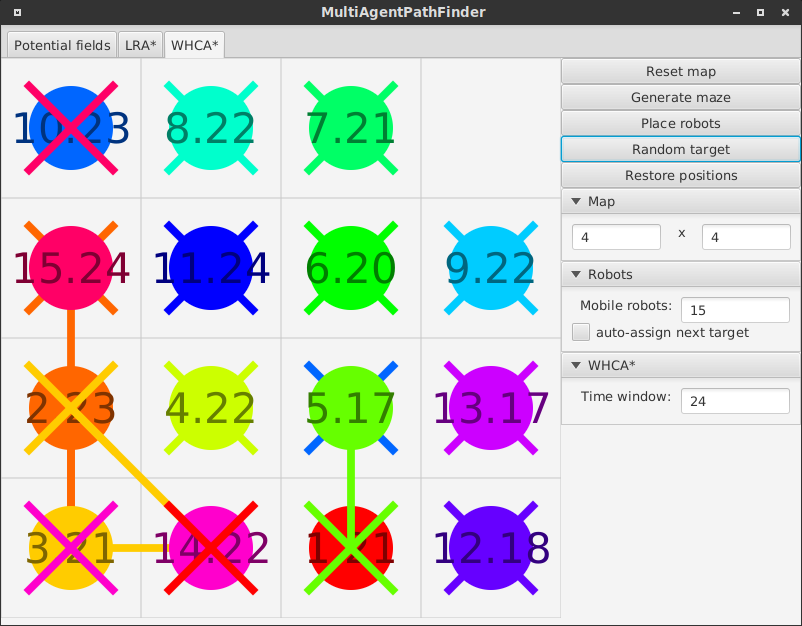
\includegraphics[width=0.8\columnwidth]{img/robopath/puzzle-15}
% 	\caption{Metoda WHCA*3: puzzle 15}
% 	\label{fig:test-puzzle-15}
% \end{figure}